% Chapter Template
\chapter{Approaches} % Main chapter title

\label{ch:03} %
The normal inference task estimate the surface normal of a 3D object. There are two main approach to solve the task. Geometry based approach estimate the surface normal of an object based on the geometry principle. Point cloud is a common surface geometry information which samples the surface point position in 3D space. Another approach is photometric stereo based approach, which utilizes a set of images under different illumination conditions. In this chapter, geometry and photometric stereo based approach are introduced separately, then a deep learning based approach using geometry information is proposed. In the end, as the main work of the thesis, another deep learning method is proposed based on both geometry and photometric stereo information.


\section{Geometry based normal estimation}


\subsection{Approach}
The geometry based normal estimation uses point cloud of the object surface as input.
Given a structured point cloud $ V^{W\times H\times 3} $ to estimate the normal map  $ N^{W\times H \times 3} $, where each normal  $ \textbf{n}^{3\times 1} $ at point $ \textbf{v}^{3\times 1} \in N $ is a unit vector with its direction point outward of the surface and perpendicular to the tangent plane of the surface at point $ \textbf{p}^{3\times 1} $.

The idea behind the neighbor based method is to fit a plane $ \Pi $ using the $ k $ neighbors $ \textbf{p}_1, ..., \textbf{p}_k \in \mathbb{R}^3 $ of the point $ \textbf{p} $, calculate the normal  $ \tilde{\textbf{n}} $ of the plane. 

It is under the assumption that the point and its neighbors are located in the same plane. This is usually not hold for the most of the surface, but if $ k $ in a suitable scale and point cloud is dense enough, it is enough to get an accurate and sharp result. As shown in Figure \ref{fig:svd-normal}. 

Specifically, it is not necessary to find the exact plane equation to solve the normal. Instead, the normal can be derived based on an equation system. 
The normal $ \tilde{\textbf{n}} $ of plane $ \Pi $ is perpendicular to all the vector on the plane $ \Pi $, we can construct $ k $ vectors on plane $ \Pi $ use  $ k $ neighbors $ \textbf{p}_1, ..., \textbf{p}_k \in \mathbb{R}^3 $ of point $ \textbf{p} $. For the simplicity, we can choose $ \textbf{p}_1 $ as the base point, then $ k-1 $ vectors can be construct as follows
\begin{equation}
	\begin{array}{rr}
		\displaystyle \textbf{v}_i = \textbf{p}_1 - \textbf{p}_i & \text{for}\ i= 2,...,k \\
	\end{array}
\end{equation}
and each of them satisfied $ \textbf{v}_i \cdot \tilde{\textbf{n}} = 0$. Then, the equation system can be constructed as 
\begin{equation}{\label{eq:normal-overdetermined-equation}}
	A \cdot \textbf{n} = 0
\end{equation}
where $ A \in \mathbb{R}^{(k-1)\times 3} $ is the vector matrix vertically stacked by $ \textbf{v}_1, ..., \textbf{v}_{k-1} $.
In order to avoid trivial solution, one more constraint should be added
\[ \|  \bn_{3 \times 1} \|_2^2 = 1  \]
which also let the normal to be a unit vector.

To calculate a valid normal, at least 3 points are required to construct, i.e. $ k>=3 $. For the sake of robust, more points can be used to reduce the measuring error. For the case $ k>3 $, since the surface vectors are actually not in the same plane, the equation system is likely over-determined . Then the equation system mentioned above can be converted to follow optimization problem
\begin{equation}
	\begin{array}{rrclcl}
		\displaystyle \min & \multicolumn{3}{l}{\| A  \bn \|^2} \\
		\\
		\textrm{s.t.} & \| \bn \|^2 & = & 1 
	\end{array}
\end{equation}
which can be solved by singular value decomposition(SVD). Let the decomposition of 
\[ A=U\Sigma V^T \]
The solution i.e. normal is the last column of $ V $.


At last, all the normals should point ot view point $ \textbf{s} $, thus the direction of a normal should be inverted if 
\begin{equation}\label{eq:normal-invertion}
	\textbf{n} \cdot (\textbf{p}  - \textbf{s}) > 0
\end{equation}

Repeat the procedure for all the points in the point cloud to get the entire normal map. 

\subsection{Evaluation}
The neighbor based method can predict the normal map in a good way when the given point cloud is dense, as shown in Figure \ref{fig:svd-normal}. It can successfully predict the smooth surface of the dragon object, especially the flakes and the tails of the dragon. 

However, it failed in the areas such as hindleg, horn and the mouth, which consists mainly by sharp edges. This is because the neighbors points in these area do not hold the assumption of coplanarity well, the normals of these neighbors can be very different. 
\begin{figure}[th]
	\centering
	\includegraphics[width=.25\textwidth]{./Figures/svd-synthetic/no-noise/fancy_eval_2_groundtruth.png}
	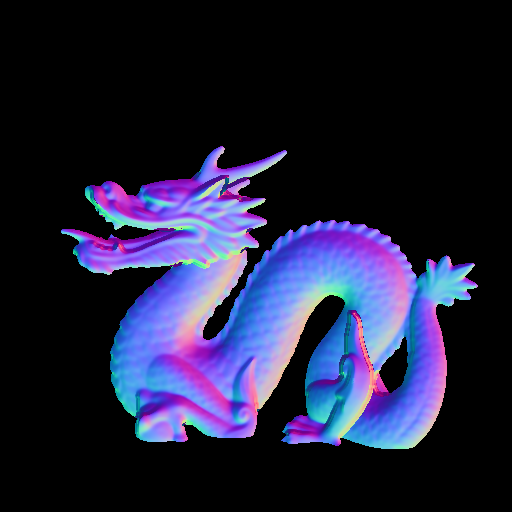
\includegraphics[width=.25\textwidth]{./Figures/svd-synthetic/no-noise/fancy_eval_2_normal_SVD.png}
	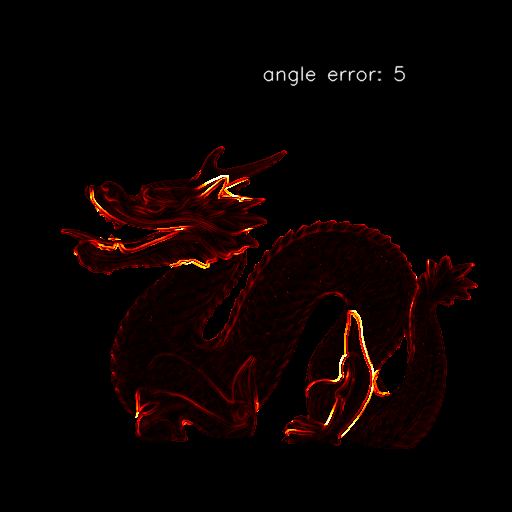
\includegraphics[width=.25\textwidth]{./Figures/svd-synthetic/no-noise/fancy_eval_2_error_SVD.png}
	
	\label{fig:svd-normal}
	\caption{Normal map of a dragon object predicted by neighbor based method. k=2, angle error=5 \textbf{Left}: ground-truth normal map \textbf{Middle}: predicted normal map, \textbf{Right}: Error map}
\end{figure}
The neighbor based method is depended on a well-chosen parameter $ k $. Figure \ref{fig:svd-k-eval} shows the evaluation on different $ k $ values. When $ k=1 $, the average error of the whole image is the lowest one, most of the normals are close to the ground-truth but the outline edges, which are the areas that surface normal changed extremely sever. For the case $ k=2 $, the sharp edges are more smooth and cause more error, like the eyes area of the dragon. Compare to the first case, the outline edge error goes better. Most of the edge errors are reduced when $ k=2 $, since more neighbor points join the evaluation and it reduces the effect of outliers. However, for the area of horn outline, hindleg outline, the error goes worse. In this case, most of the neighbors of these points are outliers and thus failed this approach.  $ k=3 $ and $ k=4 $ further increase the angle errors based on $ k=2 $.
\begin{figure}[th]
	\centering
	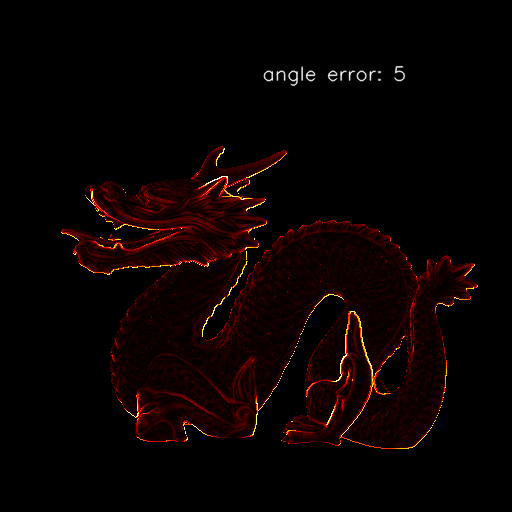
\includegraphics[width=.2\textwidth]{./Figures/svd-synthetic/k-compare/k1.png}
	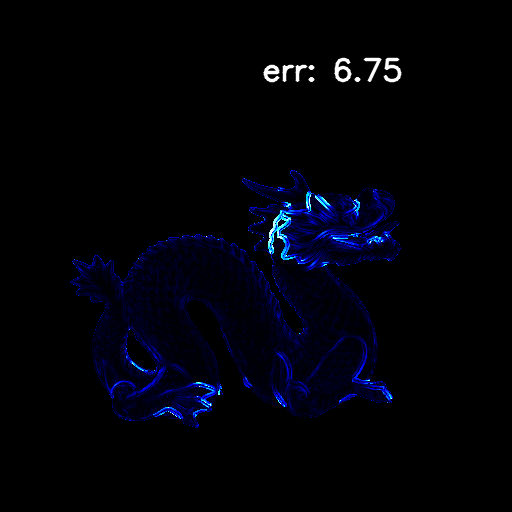
\includegraphics[width=.2\textwidth]{./Figures/svd-synthetic/k-compare/k2.png}
	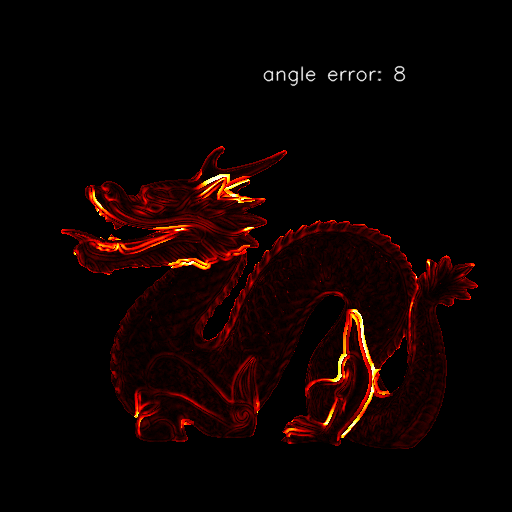
\includegraphics[width=.2\textwidth]{./Figures/svd-synthetic/k-compare/k3.png}
	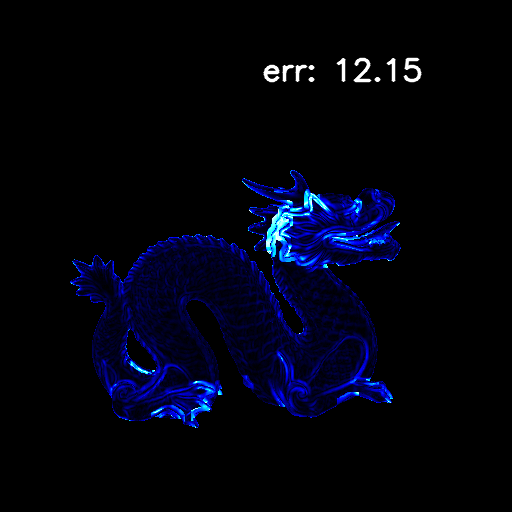
\includegraphics[width=.2\textwidth]{./Figures/svd-synthetic/k-compare/k4.png}	
	\label{fig:svd-k-eval}
	\caption{Error map of neighbor based method with different $ k $ values. From left to right, $ k=1,2,3,4 $ separately.}
\end{figure}

The performance of neighbor based method is good enough for a well chosen $ k $. However, for the case of noised point cloud as input, this approach will broken, since the noise will failed the neighbor assumption and also reduce the number of possible neighbors of each point for a fixed $ k $.
\begin{figure}[th]
	\centering
	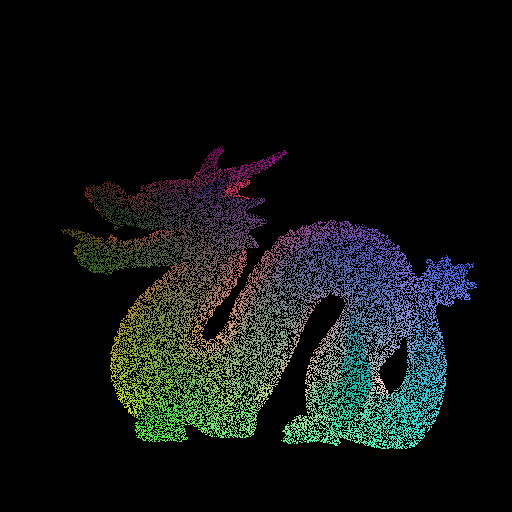
\includegraphics[width=.2\textwidth]{./Figures/svd-synthetic/noise/fancy_eval_2_point_cloud_noise.png}
	\includegraphics[width=.2\textwidth]{./Figures/svd-synthetic/noise/fancy_eval_2_groundtruth.png}
	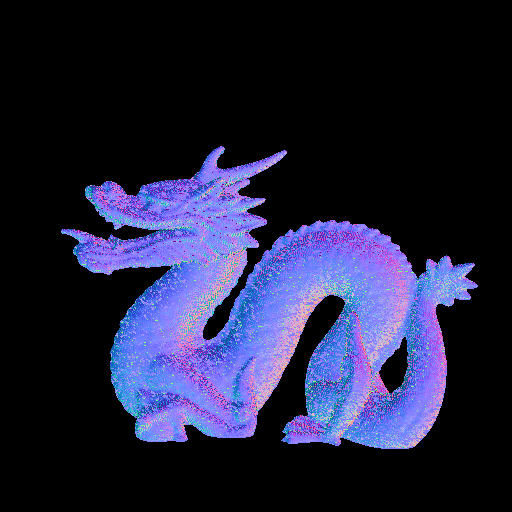
\includegraphics[width=.2\textwidth]{./Figures/svd-synthetic/noise/fancy_eval_2_normal_SVD.png}
	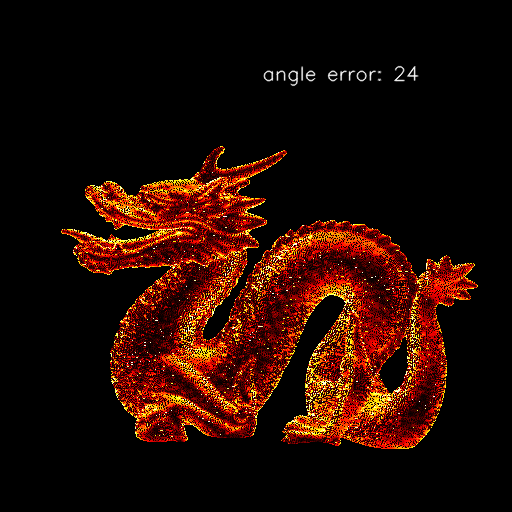
\includegraphics[width=.2\textwidth]{./Figures/svd-synthetic/noise/fancy_eval_2_error_SVD.png}	
	\label{fig:svd-noise}
	\caption{Evaluation of neighbor based method on a noised dragon model}
\end{figure}



% ---------------------- gated convolution neural network ------------------------



\section{Photometric Stereo}
Photometric stereo was initially introduced by \cite{photometric-stereo}, which estimates the surface normal of the object by observing the object in the same position but under different illuminated scenes. It based on the fact that the light reflected by a surface is dependent on the surface normal and the light direction. 

\subsection{Approaches}
Given an image $ I $, it can be decomposed in to two parts, the reflectance $ R $ and the shading $ S $,
\[ I = R\oplus S\]
where $ \oplus $ denotes the element-wise product. This decomposition of the image is based on the intrinsic image model, which proposed by  \cite{intrinsic-image}. It interprets the observed image into reflectance image and the shading image. As shown in Figure \ref{fig:intrinsic-image}
%% insert a image for decompositions
\begin{figure}[th]
	\centering
	{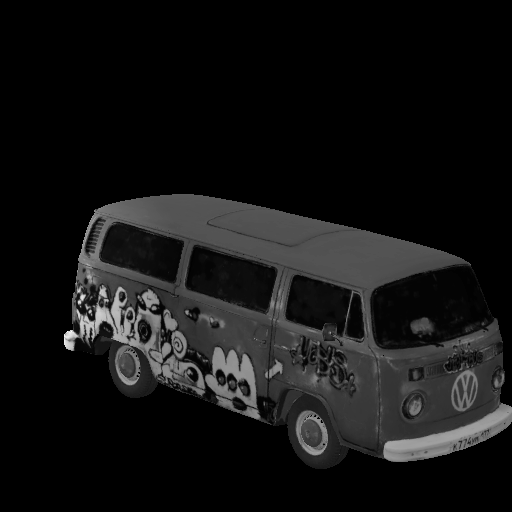
\includegraphics[width=.18\textwidth]{./Figures/intrinsic_image.png}}
	{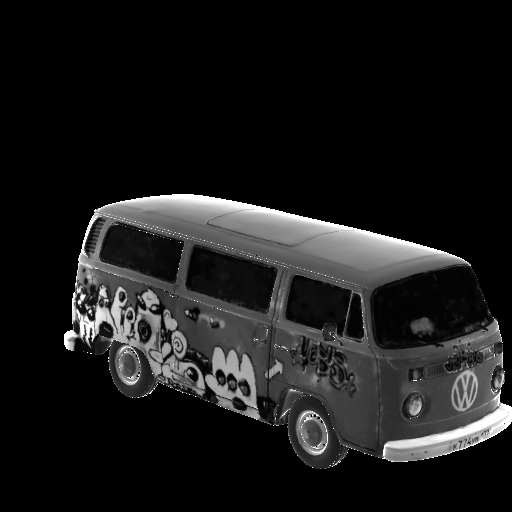
\includegraphics[width=.18\textwidth]{./Figures/intrinsic_image_reflectance.png}}
	{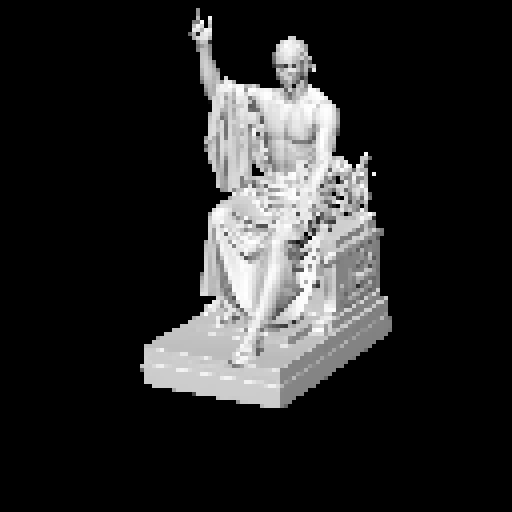
\includegraphics[width=.18\textwidth]{./Figures/intrinsic_image_shading.png}}
	{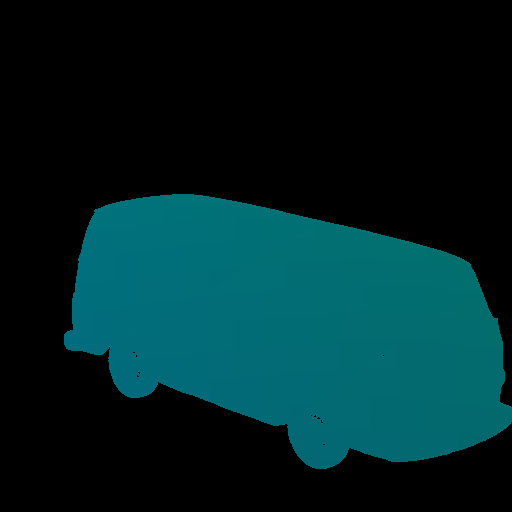
\includegraphics[width=.18\textwidth]{./Figures/intrinsic_image_light.png}}
	{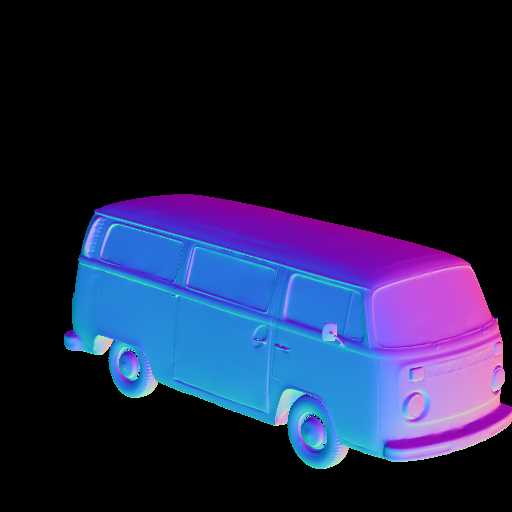
\includegraphics[width=.18\textwidth]{./Figures/intrinsic_image_normal.png}}
	\caption{Intrinsic image analysis of the bus object. From left to right, original image, reflectance image, shading image, light image, normal image}
	\label{fig:intrinsic-image}
\end{figure}

The equation can be further decomposed based on different surface models. If assume the object surfaces are Lambertian surfaces, i.e. the surface which reflect light in all directions, the shading image can be decomposed as the product of the  radiance of  incoming light $ L_0 $, the cosine of the angle of incidence, which is the dot product of the surface normal $ N $ and the light source direction $ L $.
\[ I = \rho  \odot ( L_0 \textbf{L} \cdot  \textbf{N}) \]
note that the surface normal $ N $ and light direction $ L $ are unit vectors thus they have only two degrees of freedom. 

\begin{figure}[th]
	\centering
	\begin{tikzpicture} 
		% reference lines
		\coordinate (light) at (-1,3);
		\coordinate (p) at (2,0);
		\coordinate (normal) at (2,3);
		\draw [fill=blue!20] plot [smooth cycle] coordinates {(0,0) (1,1) (3,1) (5,0) (2,-1)}; %% surface element
		\draw[thick, ->] (2,0) -- (2,3) node[midway, left] {$ \textbf{n} $}; %% normal
		\draw[thick, ->] (2,0) -- (-1,3) node[midway, left] {$ \textbf{l} $}  ; %% source direction
		\pic [draw, ->, "$\theta$", angle eccentricity=1.5] {angle = normal--p--light};
		\draw[thick, ->] (2,0) -- (5,3) node[midway, left] {$ \textbf{v} $}; %% view direction
		\filldraw[black] (-1,3) circle (2pt) node[anchor=south west]{light source}; %% light source
		\filldraw[black] (5,3) circle (2pt) node[anchor=south west]{view point}; %% view point		
	\end{tikzpicture}
	\caption{The surface normal, source light direction and the view point direction, where $ \theta $ denotes the angle between light direction and the normal.}
	\label{fig:lambertian-surface}
\end{figure}

The equation can be further rearranged as follows
\[ I = \textbf{g} \cdot \textbf{L} =(L_0\rho \odot \textbf{N}) \cdot  ( \textbf{L}) \]
The shape from shading method employed the equation mentioned above to predict the both surface albedo $ \rho $ and the normal $ \textbf{N} $ with knowning light source direction $ \textbf{L} $. More specifically, a set of $ k $ image for the same scene have been captured based on different light projections. Then, for each pixel $ (x,y) $ in the image, an equation system can be set up 

\[ 
\begin{pmatrix}
	L_1^T \\
	L_2^T \\
	\cdots \\
	L_k^T
\end{pmatrix} g(x,y) = 
\begin{pmatrix}
	I_1(x,y) \\
	I_2(x,y) \\
	\cdots \\
	I_3(x,y)
\end{pmatrix}
\]
for the simplicity, $ L_i^T $ for $ 1\le i \le k $ denotes the light direction at position $ (x,y) $ in the image $ k $ 
The equation can be solved based on least square methods. 
Since normal $ N(x,y) $ is unit vector, thus we have 

\[ \|g(x,y)\|_2 = \|L_0\rho(x,y)N(x,y)\|_2 = L_0\rho(x,y) \]

Then the normal can be obtained as follow

\[  N(x,y) = \frac{g(x,y)}{L_0\rho(x,y)}\]

In another word, the surface normal including the albedo can be obtained directly based on a set of images and light directions. 


\section{Gated Convolution neural network for surface normal estimation}
\label{sec:gcnn}


Recently, deep learning based method achieved a great succeed for image processing. ( \cite{yolov3}, \cite{efficientDet}) These network architectures use a batch of RGB / Grayscale images as input and are employed for classification problems. Usually, the images are convoluted with a convolution layer and downsampling with pooling layers. The outputs of the network consist of a single value to represent the index of the corresponding class (\cite{efficientDet}) or with a set of values to represent the position of bounding boxes.(\cite{yolov3}). However, in many other vision tasks, like normal map inference, the output is demanded as the same shape as the input. Instead of predicting one or several classes for the whole input matrix, the class for each pixel requires for prediction. In this case, the traditional network architecture is not suitable anymore.

%% upsampling 
It is worth to noticed that, the output of normal inference CNN model is not one or several labels but an entire image or normal map with same size. 
%% talk about image upsampling, unet
Recently,\cite{unet} proposed an architecture called UNet for biomedical image segmentations. The architecture is shown in Figure \ref{fig:u-net}.The first half network is a usual classification convolutional network, the second half replace the pooling layers and traditional fc layers in the traditional CNNs to upsampling layers, thus in the end of the second half, the output is able to back to the input size. The proposed network can successfully assigned each pixel a class for segmentation tasks. Under this symmetric network, an input image is downsampled 4 times and upsampled 4 times. Output image has exactly the same size as input image. The downsampling and upsampling both have large number of feature channels, which guarantee the network propagates the information to higher resolution layers.

\begin{figure}[th]
	\centering
	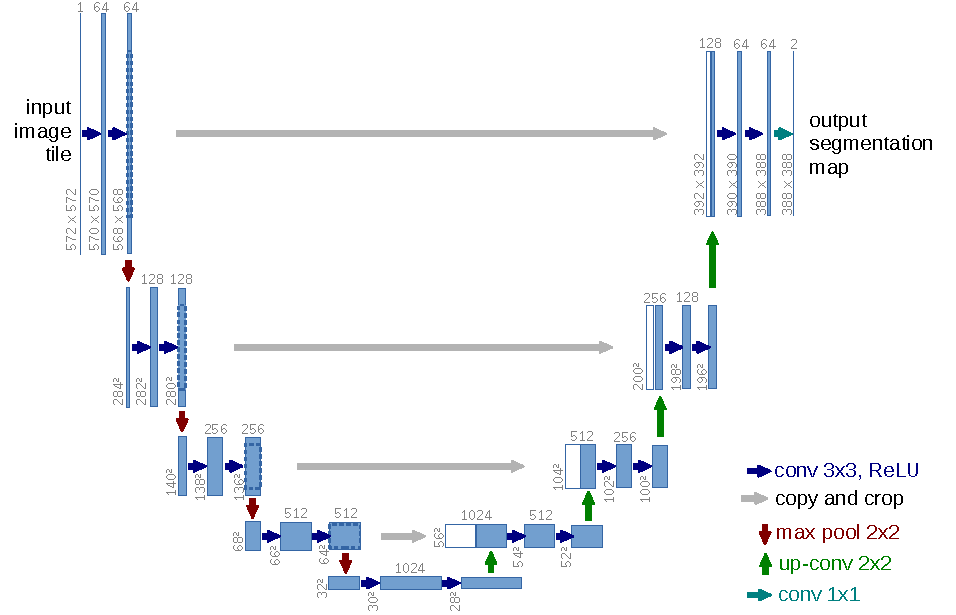
\includegraphics[width=.8\textwidth]{./Figures/u-net-illustration-correct-scale2.pdf}
	\label{fig:u-net}
	\caption{The structure of UNet. \cite{unet}}
\end{figure}


The UNet is based on standard convolution layers to construct the network. This is reasonable for image processing task with full-dense input, since no missing pixels exist. 
However, for the input of noised point cloud, the valid and invalid pixels will be treated equally if we still perform standard convolution layers. Since the aim of the network is not learning the pattern of noise, but the noise with eternally changing patterns will confuse the network, and it fails the normal inference, a mask is required to distinguish two kinds of pixels. 

% why we need a mask
\cite{pncnn0} use binary mask to indicate valid pixels, and further use normalized convolution to predict the output. The normalized convolution is shown as follows

\begin{equation}
	\begin{array}{rrclcl}
		O(x,y) = 
		\begin{cases}
			\dfrac{\Sigma_i^k\Sigma_j^k W(i,j) \cdot I(x-i,y-j) \cdot M(x-i,y-j)}{\Sigma_i^k\Sigma_j^k W(i,j) \cdot M(x-i,y-j)}, & \text{if}\ \sum_{i}^k\sum_{j}^k M(i,j)>0 \\
			0, & \text{otherwise}
		\end{cases}
	\end{array}
\end{equation}

where $ k $ is the kernel size, $ (x,y) $ is the position in input, $ (i,j) $ is the displacement in kenel, $ M $ is the corresponding mask. A binary mask uses 1 to indicate valid pixels and 0 otherwise. $ \odot $ denotes element-wise multiplication.

Normalized convolution layer added the weight to the mask. However, a initialization for the mask is still required, and the propagation of the mask remain a tricky task. 

\subsection{Gated Convolution}

% introduce gconv
\cite{gated_activation} proposed a gated activation unit to model more complex interactions comparing to standard CNN layers, which mainly inspired by the multiplicative units exist in Long Short-Term Memory proposed by \cite{lstm} and Rated Recurrent Unit (GRU) proposed by \cite{gru}. 
\cite{gconv} employed the same gated unit solving for the free-form image inpainting task. The proposed network use 3 channel RGB images as input and estimate the missing pixels. 


The structure is shown in Figure \ref{fig:gconvLayer}. Instead of using a mask as input to indicate valid pixels, it employs a standard convolution layers to learn this mask directly from data. The valid pixels are then activated by a Sigmoid function. Then it imply element-wise multiplication with the feature map. Formally, the gated convolution is described as follows, the layer with input size $ (N, C_{in}, H, W) $ and output size $ (N, C_{out}, H_{out}, W_{out}) $:
\begin{equation}\label{gconv}
	o(N_i, C_{o_j}) = \sigma(\sum_{k=0}^{C_{in}-1}w_g(C_{o_j}, k) \star i(N_i,k) + b_g(C_{o_j})) * 
	\phi (\sum_{k=0}^{C_{in}-1}w_f(C_{o_j}, k) \star i(N_i,k) + b_f(C_{o_j}))
\end{equation}
where $ \phi $ is LeakyReLU function, $ \sigma $ is sigmoid function, thus the output values are in range $ [0,1] $, $ \star $ is the valid 2D cross-correlation operator, $ N $ is batch size, $ C $ denotes a number of channels, $ H $ is a height of input planes in pixels, and $ W $ is width in pixels, $ w(C_{o_j},k) $ denotes the weight of $ j $-th output channel corresponding $ k $-th input channel, $ i(N_i, k) $denotes the input of $ i $-th batch corresponding $ k $-th input channel, $ b(C_{o_j}) $ denotes the bias of $ j $-th output channel.


% Gated Convolution Layer
\begin{figure}[th]
	\centering
	\begin{tikzpicture}
		\tikzstyle{rect} = [rectangle, rounded corners, minimum width=3cm, minimum height=1cm,text centered, draw=black, fill=blue!20]
		\tikzstyle{arrow} = [thick,->,>=stealth]
		\node (output) [rect] {Output};
		\node (oplus) [below of=output, yshift=-.2cm] {$\Huge\oplus $};
		\node (LeakyReLU) [rect,below of=oplus, yshift=-0.4cm] {Feature};
		\node (sigmoid) [rect, below of=oplus, yshift=-0.4cm, xshift=-4cm] {Mask};
		
		\node (conv1) [rect,below of=sigmoid, yshift=-1cm] {Mask};
		\node (conv2) [rect,below of=LeakyReLU, yshift=-1cm] {Feature};
		\node (input) [below of=oplus] at (0,-7) {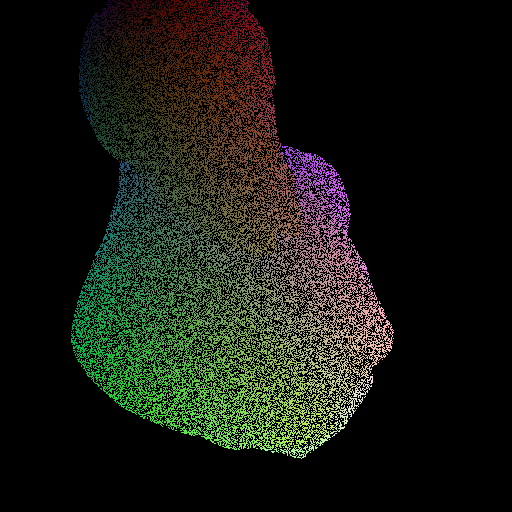
\includegraphics[width=.25\textwidth]{./Figures/train-input.png}};
		
		\draw [arrow] (oplus) -- (output);
		\draw [arrow] (sigmoid) |- (oplus);
		\draw [arrow] (LeakyReLU) -- (oplus);
		\draw [arrow] (conv2) --  node [text width=2.5cm, midway, right=1em]{LeakyReLU} (LeakyReLU);
		\draw [arrow] (conv1) --  node [text width=2.5cm, midway, right=1em]{Sigmoid} (sigmoid);
		\draw [arrow] (input) -|  node [text width=2.5cm, midway, below=1em]{Conv2D} (conv1);
		\draw [arrow] (input) -- node [text width=2.5cm, midway, right=1em]{Conv2D} (conv2);
	\end{tikzpicture}
	\caption{Gated Convolution Layer, where $ \oplus $ denotes element-wise multiplication.}
	\label{fig:gconvLayer}
\end{figure}

%\section{Canny Edge Detection for Detail Enhancement}
%The inaccuracy part is usually concentrate in the coarse surface or drastic changed surface parts of the object. The corresponding part can be extracted separately via edge detector algorithms, like Canny Edge detector. Feed the edges to a special net for normal prediction might improve the accuracy further. 

\subsection{Architecture}
\label{sec:architecture}
Based on the implementation mentioned above, the architecture roughly follows on UNet proposed by \cite{unet}, as shown in Figure \ref{fig:gcnn-archi}. 

\begin{sidewaysfigure}[th]
	\centering
	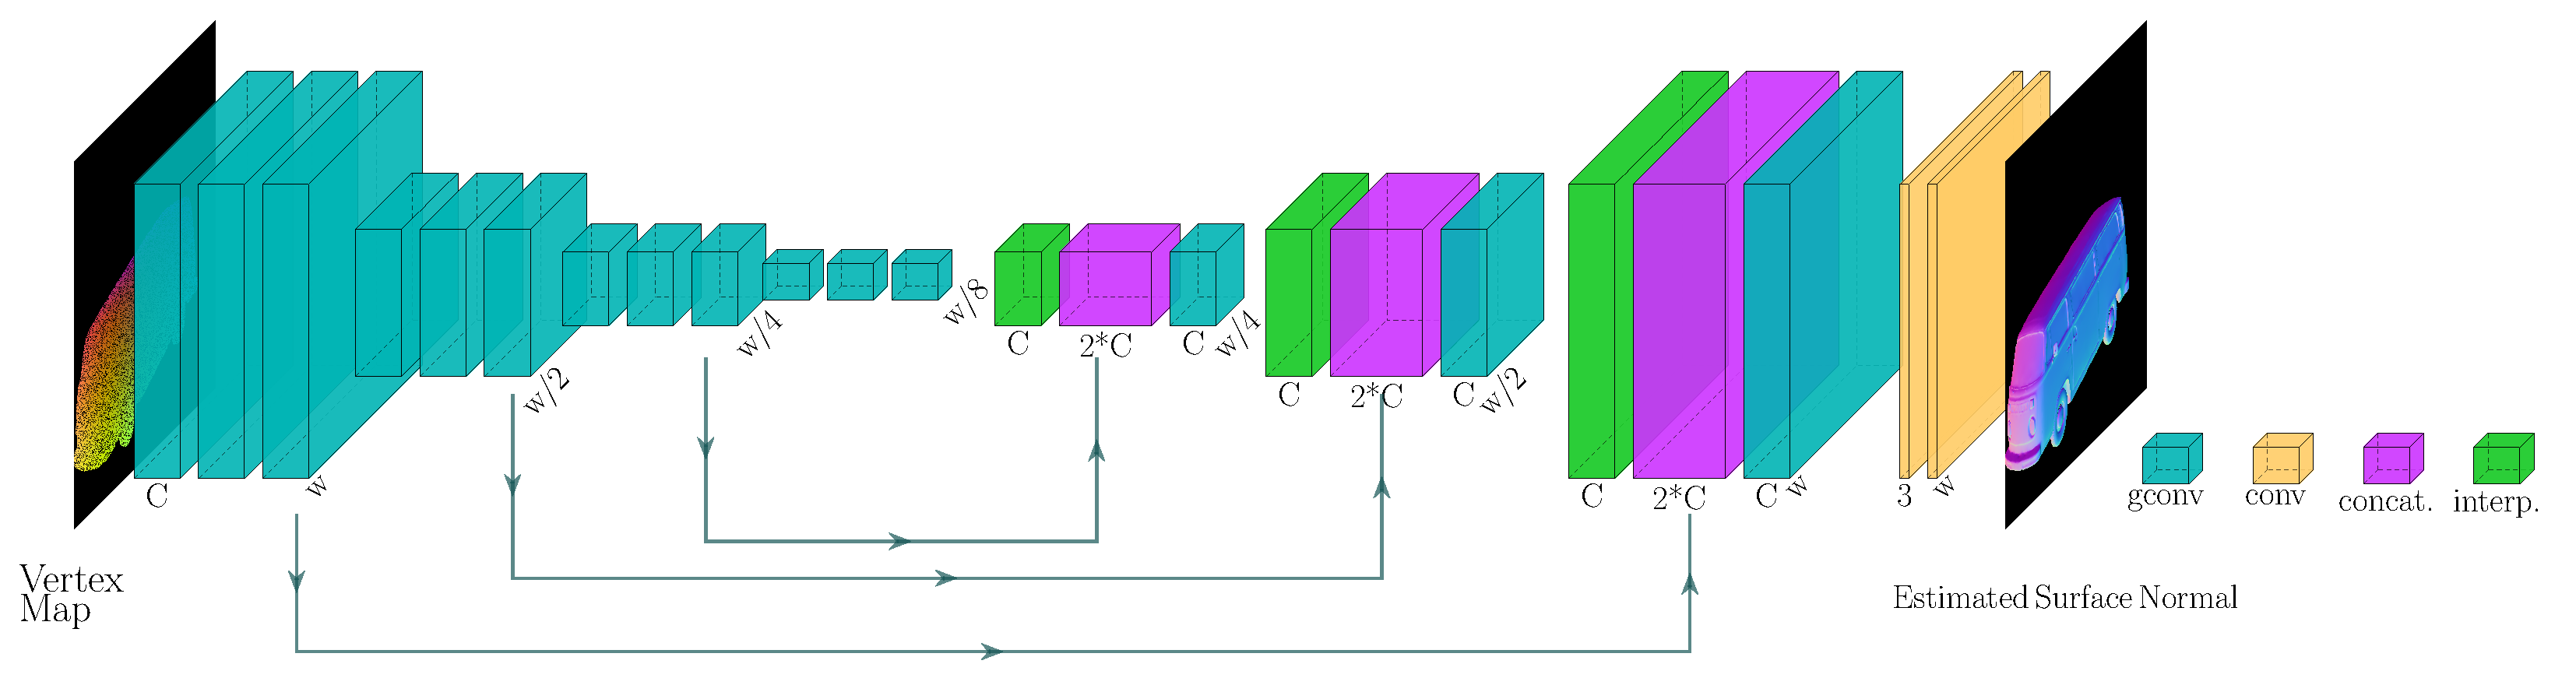
\includegraphics[width=1\textwidth]{Figures/gcnn}
	\caption{The architecture of Gated convolution neural network (GCNN) based on Gated convolution and UNet Architecture.}
	\label{fig:gcnn-archi}
\end{sidewaysfigure}
In order to describe the network in a common way, the parameters of the network are represented by letters.
The network is constructed by a downsampling part and a upsampling part. In the downsampling part, the input is the $ X \in \mathbb{R}^{w\times w\times ch}$. The input matrix goes through 3 downsampling layer blocks, each block has two gated convolution layers with stride (1,1) and an extra gated convolution layers with stride (2,2) as a downsampling operation. 
The total three times downsamplings extract the geometry features $ X_v $ from input matrix $ X $ (represented as a regression function $ f $)
\[ f: X \rightarrow X_f \]
After the feature extraction, the network upsampling the feature map 3 times to get the output matrix $ Y $. Each upsampling consists of an interpolation operation uses nearest neighboring interpolations for resolution upsamling, then a concatenate layer that concatenate the interpolated result and the corresponding high resolution feature map  $ X_{df_1, df_2, ...} $  from the downsampling part. This is also called skip connection. In the last, a gated convolution layer is utilized to reduce the channel size to fit the next upsampling block. After the three times upsampling, two standard convolution layer is added in the last without activation function to predict the surface normal. The whole upsampling branch can be represented as a regression function $ n $,
\[ n: X_v, X_{df_1, df_2, ...} \rightarrow N \]
All the convolution layers in the network use same kernel size $ 3\times 3 $. 

One of the key feature of the network is the output has the same size as the input. This is achieved by the (1,1) padding and the same channel number in the convolution layers. Thus the surface normal can be achieved 1-1 estimation. Another key point of the network is the robustness of the noise. The network takes semi-dense matrix as input then predicts the fully-dense matrix as output. The last feature is the multi-purpose using scenarios. In the description, no specific input type has been indicated. In this thesis, two application scenarios have been verified. The first is the missing-pixel estimation but with out the transformation of the style of the input matrix, which takes the semi-dense matrix as input and simply fill the missing pixels in the output. The second is the missing pixel estimation with style-transferred of the matrix. In this case, the network takes the semi-dense matrix as input, the output matrix is fully-dense but each pixel has the different meaning as the input. Actually, the first scenario can be consider as the specially case of the second scenario which the style of output and the input remain the same. The network is test in Chapter \ref{ch:05}, which is shown the good performance on noise filtering task and also the normal surface estimation task.

\subsection{Loss Function}

\paragraph{L1 Loss}
L1 loss, also known as absolute error loss, which calculates the absolute difference between the prediction and the ground truth. It leads to the median of the observations.

\[ L_1(\tilde y - y) = |\tilde y - y | \]

\paragraph{L2 Loss}
The standard loss function for optimization in regression problems is the L2 loss, also known as squared error loss, which minimize the squared difference between a prediction and the actual value. It leads to the mean of the observations. 
\[ L_2(\tilde y - y) = \|\tilde y - y \|_2^2 \]


\paragraph{Masked L2 Loss with penalty for outliers(mask-l2)}
\label{par:maskl2}
The background pixels of the input data are not considered in the normal inference task, they are saved as black pixels in the input data. These pixels should not considered in the loss function, i.e. invalid pixels. Therefore, a valid mask is required to distinguish the background and the main object. Specifically, using a matrix with the same width and height as the output, for each pixel, 0 is invalid, 1 is valid. 
Furthermore, depends on the specific task, the output should be constraint in a range. For normal output, the range is $ [-1,1] $. Thus for the outliers out of this range, a outlier mask can be applied to give them a penalty.

\begin{equation}\label{gcnn-loss}
	\begin{array}{ll}
		l(x,y)&= L  = \{l_1, ..., l_N\}^T\\ 
		l_{n\in N} &= \| mask_{obj} \odot mask_{ol} \odot ( {\tilde y}_n - y_n) \|_2^2 + 	\| mask_{obj} \odot mask_{nol} \odot ( {\tilde y}_n - y_n) \|_2^2 \\
	\end{array}
\end{equation}

where $ x $ is input, $ y $ is target, $ N $ is the batch size.$ mask_{obj} $ is the mask of the object, i.e. 1 means it is an pixel on the object, 0 is an pixel on the background. $ mask_{ol} $ is the mask for the outliers, i.e. 1 means outliers, 0 means non outlier, $ mask_{nol} $ is exactly the inverse of $ mask_{ol} $. $ p $ is the penalty of the outliers, it is set as 1.4.


\paragraph{Reversed Huber Loss}

\cite{berhu-loss} proposed Reversed Huber loss to combine both L1 and L2 loss. L1 loss is for small values whereas L2 for large values
\begin{equation}\label{berhu-loss}
	\begin{array}{ll}
		\mathcal{B}(y)= \begin{cases}
			|y| & |y| \le c \\
			\dfrac{y^2 + c^2}{2d} & |x| > c\\
		\end{cases}
	\end{array}
\end{equation}
where $ c=0.2\max (|\tilde y - y|) $.


\section{Guided normal inference using GCNN}
The guided normal inference takes the light direction and the image into consideration. It is under the assumption that the scene image $ I $ is captured by a calibrated camera, i.e. knowing the intrinsic $ K $ and extrinsic camera matrix $ [R|t] $, and a the light position $ (s_x, s_y, s_z) $ of the single light source. The geometry based approach inference the surface normal from the point cloud, whereas the photometric stereo inference the surface normal from a set of calibrated illuminated images. The idea behind this chapter is that improve the geometry based approach with the help of one calibrated illuminated image. Since the calibrated illuminated image contains the information about the surface feature, it is supposed to help the geometry approach in a proper way. Based on this idea, two networks are proposed in this section.

\subsection{Light Map}
\label{sec:lightmap}
The light map $ L $ can be derived from vertex map $ V $ and the light source position $ s $. As shown in Figure \ref{fig:lambertian-surface}, the incoming light direction is a vector point from light source to the surface point, therefor it can be calculated as follows
\begin{equation}\label{light-direction}
	\begin{array}{ll}
		L(x,y)&= \dfrac{V(x,y)-(s_x,s_y)}{\|V(x,y)-(s_x,s_y)\|_2}\\ 
	\end{array}
\end{equation}
\begin{figure}[H]
	\centering
	{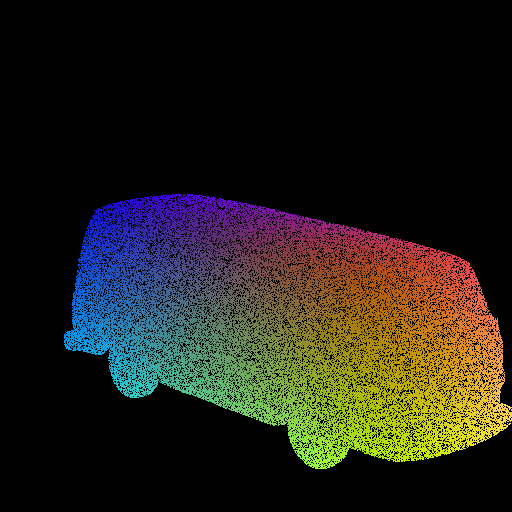
\includegraphics[width=.25\textwidth]{./Figures/intrinsic_image_vertex_input.png}}
	{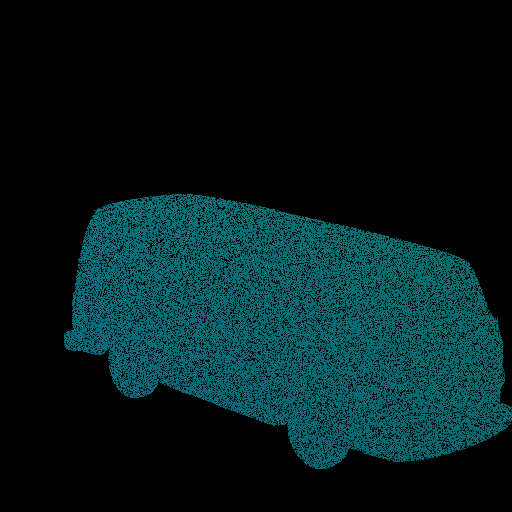
\includegraphics[width=.25\textwidth]{./Figures/intrinsic_image_light_input.png}}
	\caption{The light map calculated from vertex map and the light source}
	\label{fig:light-input}
\end{figure}
where $ (s_x,s_y) $ is the light source position and $ V $ is the vertices, both $  (s_x,s_y) $ and  $ V $ are with respect to the camera space. The light direction map $ L $ is normalized since only the direction of the light is considered. Using the equation above for all the pixels in the point cloud can obtain the corresponding light map, which is a matrix with same size as point clouds. However, it is important to note that due to the exist noise in the vertex map, the getting light map is only semi-dense, as shown in Figure \ref{fig:light-input}. 





\subsection{VIL Net}
Based on above implementations, we propose a light and image guided network called Vertex-Image-Light Network (VIL-Net). The structure is basically derived from GCNN model as mentioned in \ref{sec:gcnn}, which is shown in Figure 
\ref{fig:VIL-Net}.

As mentioned in the name, the \textbf{VIL}-Net utilizes \textbf{V}ertex map, \textbf{L}ight map and \textbf{I}mage map to accomplish the normal inference task. 

The network can be consider in two parts. The first part extracts the feature maps from the input data. It deals with two kinds of input, the vertex map $ X_1 \in \mathbb{R}^{w\times h\times3}$, and the concatenation of light and image map $ X_2 \in \mathbb{R}^{w\times h\times4} $. The network extracts the geometry features $ X_v $ from vertex map $ X_1 $ (represented as a regression function v)
\[ v: X_1 \rightarrow X_v \]
and the photometric features $ X_l $ from image and the light map $ X_2 $ (represented as a regression function $ l $)
\[ l: X_2 \rightarrow X_l \]
where the two encoders have the same network architecture based on the downsampling part of GCNN model. After the feature extraction, 2 extra layers are added: 1, a concatenate layer is added to fuse the vertex feature, and the image and light map feature getting from the encoder. 
2, a fused feature map is predicted from all the feature maps base on a single gated convolution layer. (represented as a regression function $ m $)
\[ m: [X_v X_l] \rightarrow X_f \]
Then the network interpolates the feature maps $ X_f $ 3 times using interpolation and gated convolution layers to inference the normal map $ N $. Meanwhile, the skip connections fuse the high resolution features $ X_{df_1, df_2, ...} $ from the downsampling part during the upsamplings. The upsampling is represented as a regression function $ n $:
\[ n: X_f, X_{df_1, df_2, ...} \rightarrow N \]

With the help of an extra image-light encoder, the network gained more information of the object surface, which is supposed to predict the surface normal more accurate. In this scenario, the output is still the surface normal, thus the training loss can be the same as GCNN model.


\begin{sidewaysfigure}[th]
	\centering
	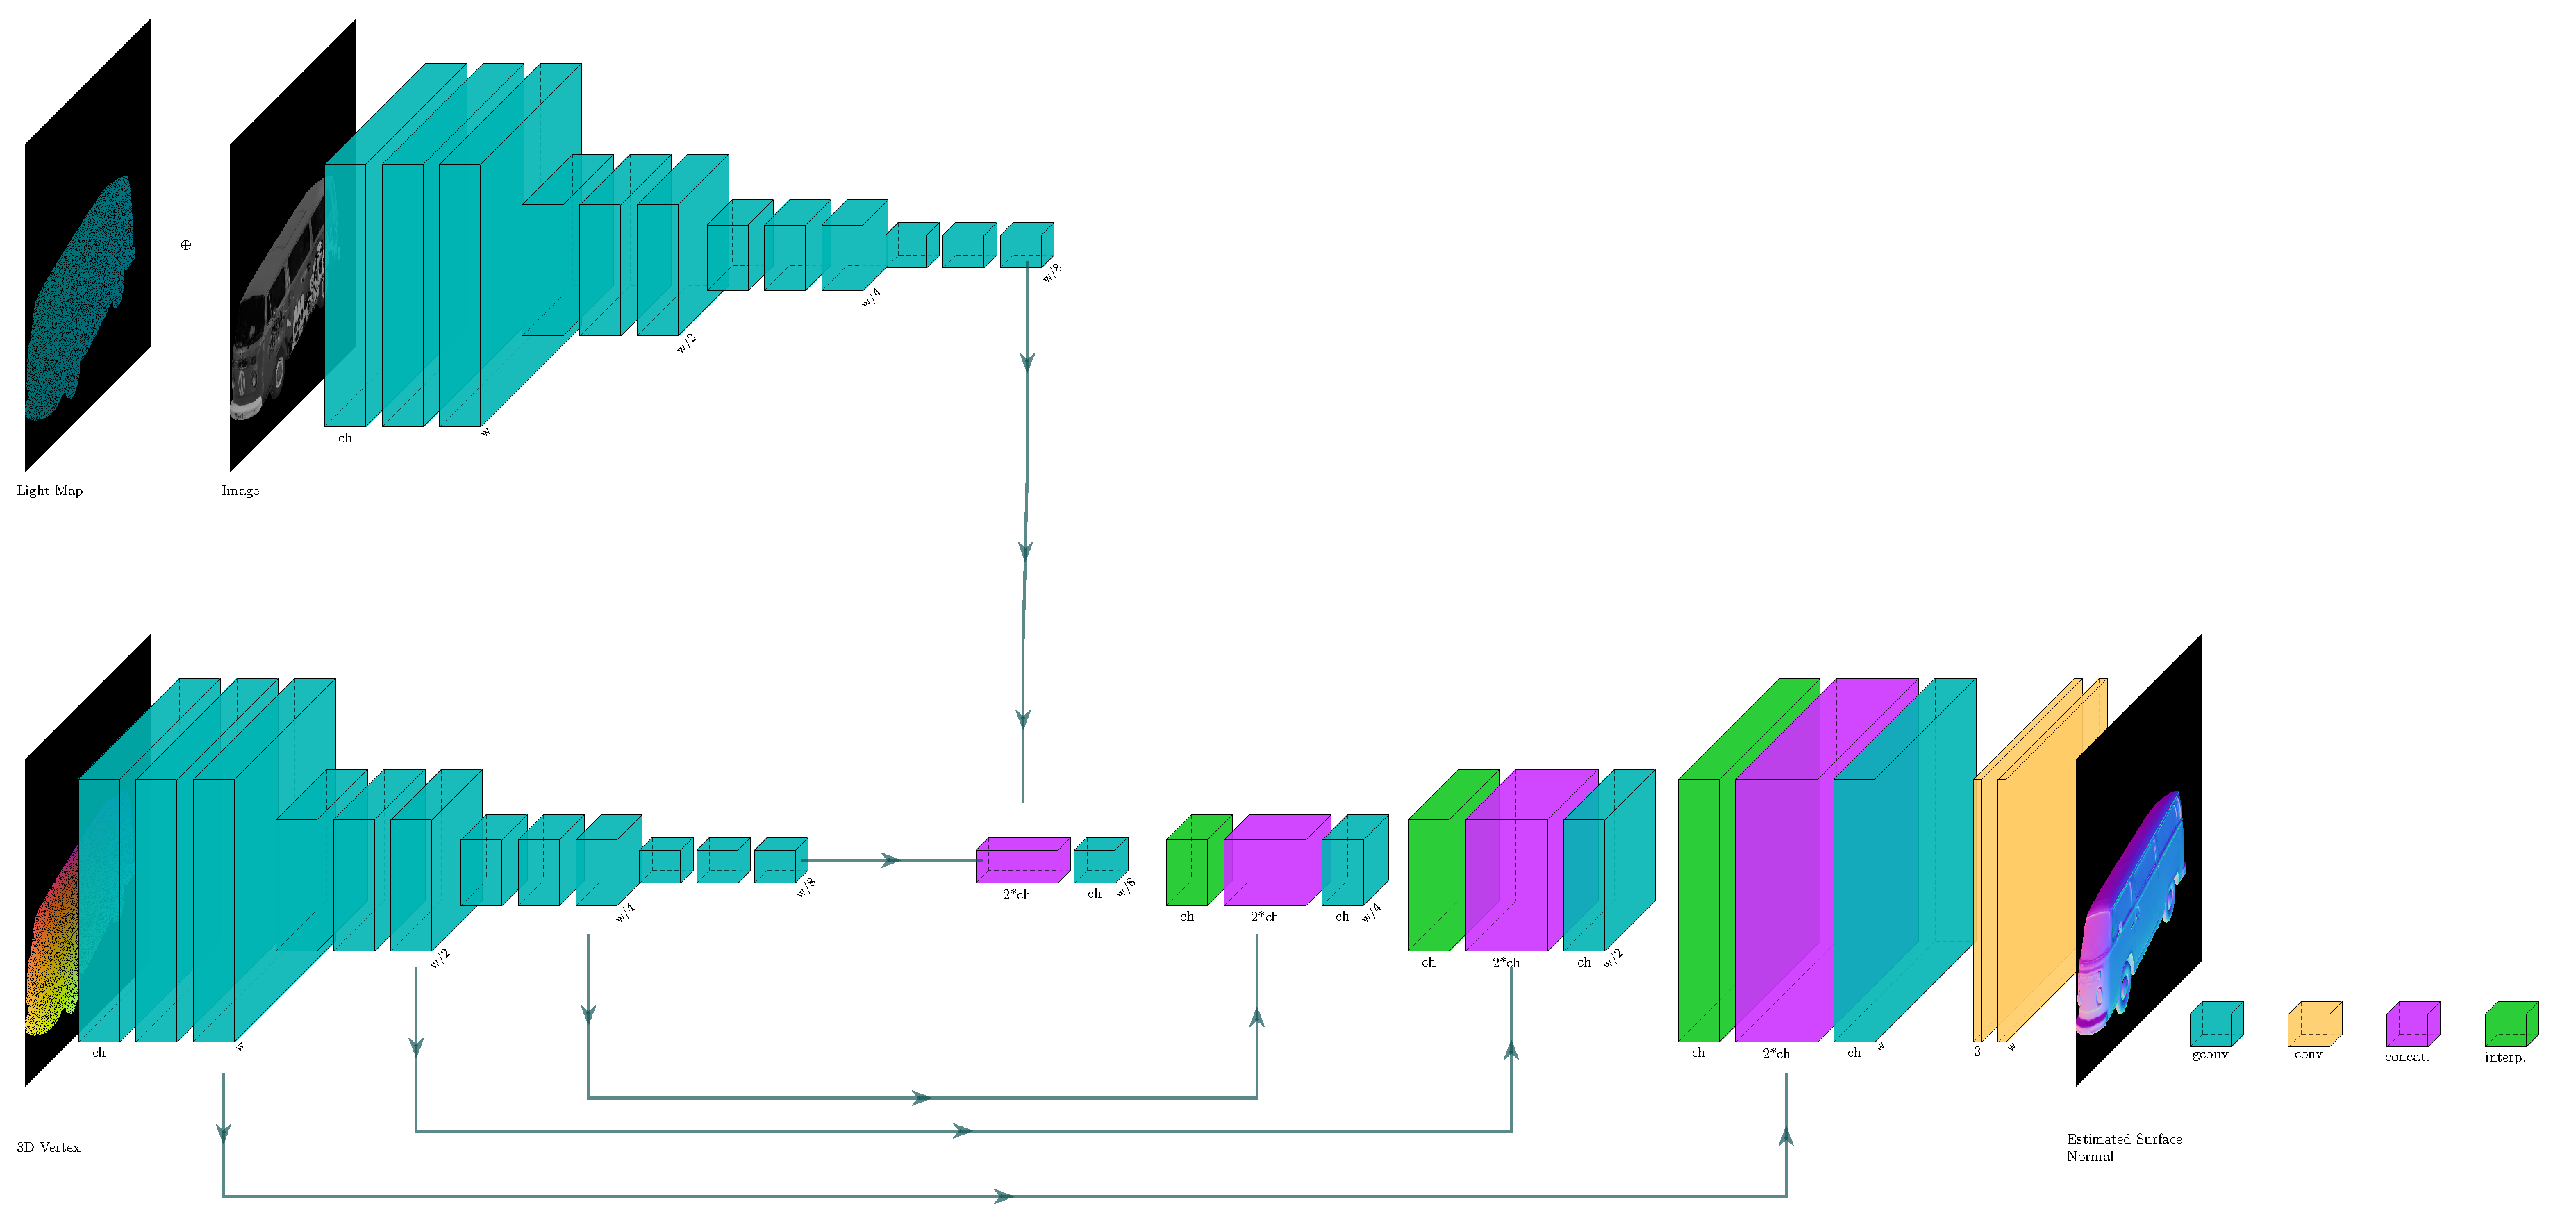
\includegraphics[width=1\textwidth]{Figures/vil-net} % Research group name and department name
	\caption{The architecture of VIL-Net}
	\label{fig:VIL-Net}
\end{sidewaysfigure}


\subsection{TriG-Net}

We propose a light and image guided network called Triple-pipe-gated-Network (Trip-Net), which employs the GCNN architecture three times to accomplish the normal inference task. The architecture is shown in Figure \ref{fig:Trig-Net}.

The network has three pipes combined with one main pipe and two side pipes. Each pipe deals with different task. The main pipe deals with the geometry information, which takes the vertex map as the input and used to predict the surface normal. The light map is fed into a side pipe and used to extract the light feature. The network forwards the features to the main pipe as a supplementary information for the normal estimation. The image pipe takes the image as the input and extracts the image features then forward the features to the main pipe as well. The supplementary pipes provide the illumination information which helps the main pipe to refine the inferred normals.
\subsubsection{Side-Pipe(Light)}
The task of light pipe in the network is to predict the light feature from the photometric information using the light direction in the scene, which is calculated from the point cloud and the light position. The light map also inherits the noise from the point cloud, which lead to a semi-dense input map. Therefore this side pipe utilizes gated convolution layers for feature map extraction to handle the missing values. The input vertex map is downsampled three times in this part. Each downsampling utilizes three gated layers, the first two layers have stride (1,1) and the third one has stride (2,2) to reduce the feature scale. 
In the upsampling part, the network also has three times upsampling as a symmetric design. In each upsampling, it first uses nearest neighbor interpolation algorithms to expend the feature map size. Then it concatenates the corresponding feature map from the downsampling part. In the last, the feature map goes through a gated convolution layer to reduce the channel size. 

\subsubsection{Side-Pipe(Image)}
The task of image pipe in the network is to predict the image feature. This pipe is a collaborate pipe with the light pipe. The architect is the same as light map pipe but only the input is the image matrix. 


\subsubsection{Main-Pipe(Vertex)}
The task of vertex pipe in the network is to predict the normal map directly. The input is vertex map converted from point cloud. The downsampling part is still the same as the other two pipes. The different part is the upsampling, which has to consider the information coming from the other two pipes. After the downsampling, a concatenation layer fused the corresponding feature map from the other two pipes, then it takes 3 times upsampling. Each upsampling consists of 5 layers: 1, a interpolation layer to double size the resolution using nearest neighboring interpolation algorithm, 2, a gated layer to reduce the channel size to 1/3 of itself in order to fit the corresponding feature map in the downsampling part, 3, a concatenation layer to fuse the output with the corresponding feature map in the downsampling part, 4, a gated layer to reduce the channel size to 1/2, 5, a concatenation layer to fuse the corresponding upsamling feature map from the other two pipe altogether with the feature map in current pipe. These 5 layers consider both the information from other pipes and also keeps the high resolution from the downsampling part. A gated convolution layer is added afterwards to reduce the channel size and extra two standard convolution layers are used to predict the final surface normal map.


\begin{sidewaysfigure}[th]
	\centering
	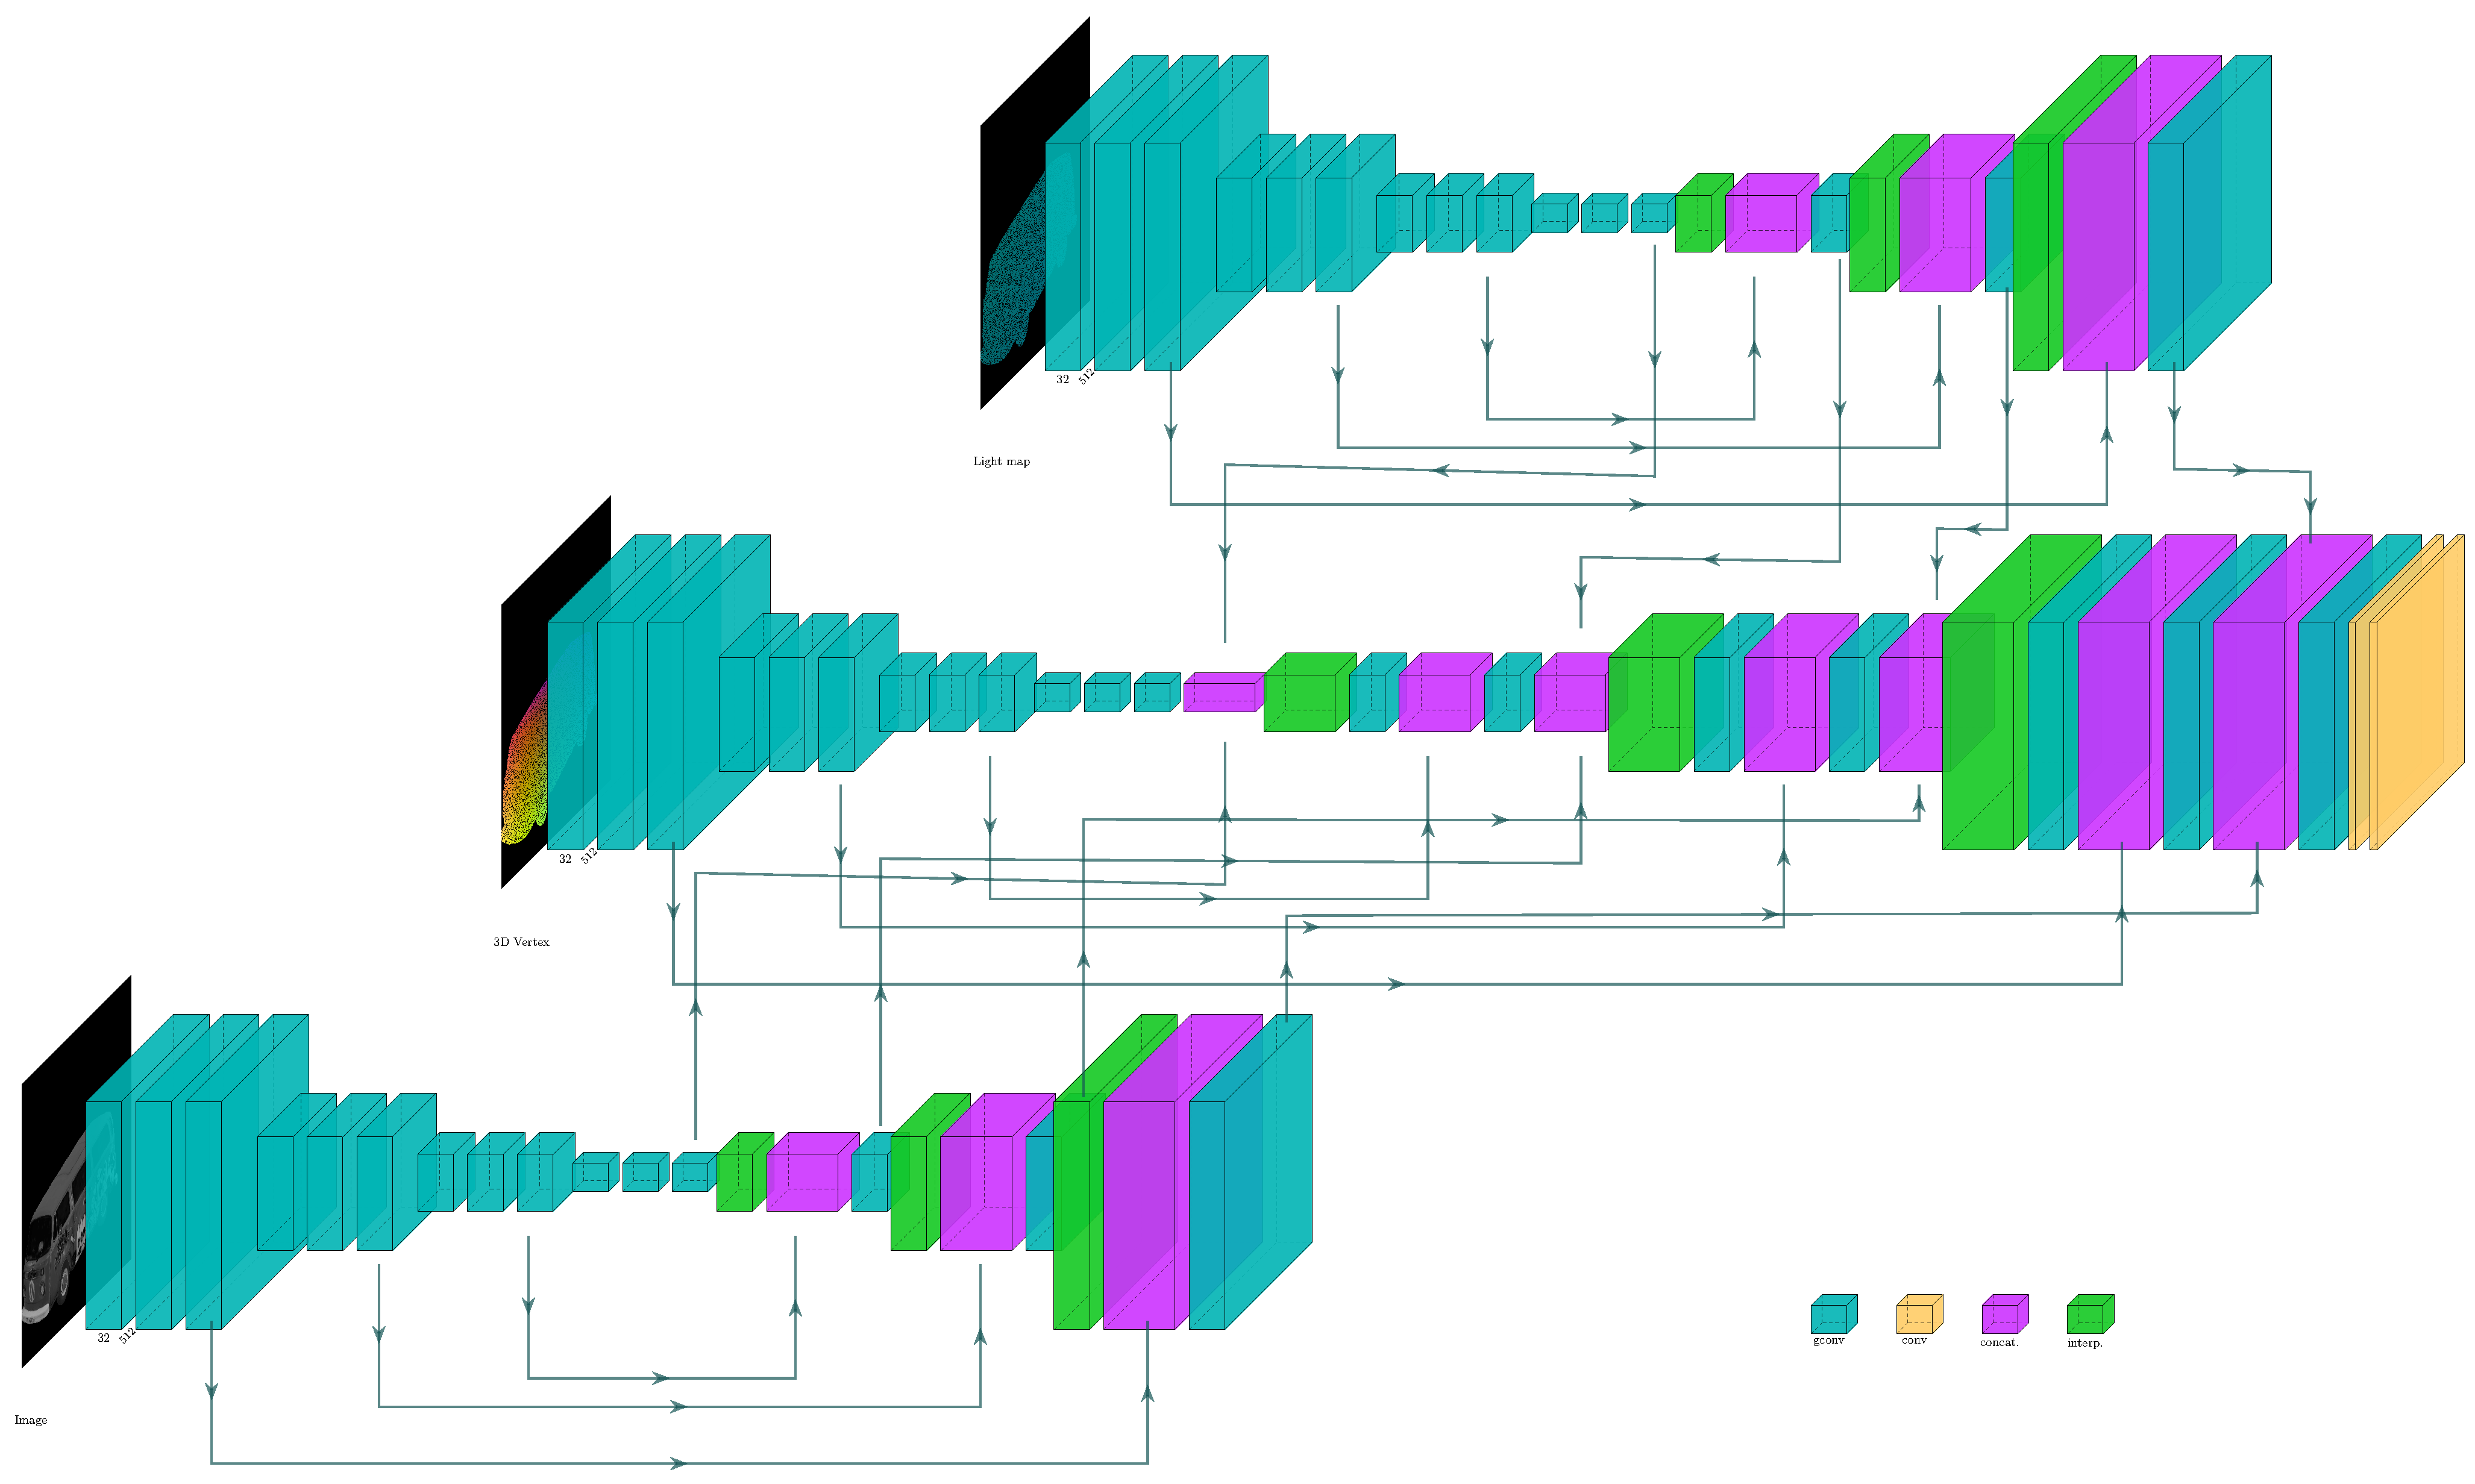
\includegraphics[width=1\textwidth]{Figures/trignet} % Research group name and department name
	\caption{The architecture of Trig-Net}
	\label{fig:Trig-Net}
\end{sidewaysfigure}






